\documentclass[a4paper]{article}

%% Language and font encodings
\usepackage[english]{babel}
\usepackage[utf8x]{inputenc}

\usepackage{booktabs}
\usepackage{tabu}
\usepackage[T1]{fontenc}

%% Sets page size and margins
\usepackage[a4paper,top=3cm,bottom=2cm,left=3cm,right=3cm,marginparwidth=1.75cm]{geometry}

%% Useful packages
\usepackage{amsmath}
\usepackage{xfrac}
\usepackage{graphicx}
\usepackage[colorinlistoftodos]{todonotes}
\usepackage[colorlinks=true, allcolors=blue]{hyperref}
\usepackage{caption}

% Package for writing pseudo code
\usepackage{algorithmic}

% Start each section in a new page
\usepackage{titlesec}
\newcommand{\sectionbreak}{\clearpage}

% Path to images directory
\graphicspath{{images/}}

%\title{Motion simulation of autonomous surface vehicle in irregular sea using
%frequency domain analysis}
%\author{Toby Thomas \small{(CEng, MBCS, MRINA)}}
%\date{\today}

\begin{document}
%\maketitle

% Insert table of contents
\tableofcontents

\section{Ocean Waves} \label{Ocean Waves} 
This document presents a summary of the theory of ocean waves and is mainly 
based on \cite{lewis1988principles}.

The outstanding visible characteristic of an open sea surface is its
irregularity. The waves on the surface do not repeat periodically in time or
space. Yet, over a wide area and for a period of time, the sea surface maintains
a characteristic appearance. Study on wave data have shown that even though the
sea surface is irregular, the wave elevation readings is Gaussian in nature and
is statistically a constant for a given area for a certain period of time. It is
therefore possible to define a sea condition, for a region for a (short) period
of time, using statistical parameters such as mean elevation and variance. The
mean elevation will however be zero, since wave does not change the water level
in the sea. Which means, considering Gaussian distribution for wave elevations,
the sea condition can be defined using variance alone.

For the purpose of this research we consider waves generated due to storms, that
is waves that are generated by the interaction of wind and water surface. The
two main physical process involved in the generation of storm waves are the
friction between air and water and the local variation of pressure field due to
wind. Even though there are many processes that will affect the growth and
propagation of waves, for waves of small amplitude, it is primarily governed by
the principle of superposition. So if $\zeta_1(x,y,t)$ and $\zeta_2(x,y,t)$ are
functions that represent two wave systems then $\zeta_1(x,y,t) + \zeta_2(x,y,t)$
is also a wave system.  However, it should be noted that the assumption
regarding the linear superimposability of waves fails when the wave system is
too steep and wave breaking occurs.

\subsection{Regular sea waves} \label{Regular sea waves}

A regular sea wave is a harmonic wave with crests that are infinitely long,
parallel and equally spaced and having constant wave heights. The general 
equation of a regular long crested wave travelling at a angle $\mu$ to the 
$x$-axis is:
\begin{equation}
  \zeta (x,y,t) = \zeta_a \cos[k(x \cos \mu + y \sin \mu) - \omega t + \epsilon]
  \label {eq: 2D wave equation}
\end{equation}
where: \\ 
$\zeta_a$ is the wave amplitude at the water surface\\ 
$k = \frac{2 \pi}{L_w}$ is called the wave number.\\ 
$L_w$ is the wave length\\ 
$x$ is the distance along the x-coordinate\\
$y$ is the distance along the y-coordinate\\
$\mu$ is the direction of propagation of the wave as an angle with respect to
positive direction of x-axis.\\
$\omega$ is the circular frequency of the simple harmonic wave\\
$t$ is time\\
$\epsilon$ is a phase angle. 


The wave system travels perpendicular to the line of crests with a velocity
$V_c$. It is assumed that water is incompressible and has zero viscosity. Based
on these assumptions the motion of water particle in the wave can be described
using a quantity called \textit{velocity potential} which is defined as a function
whose negative derivative in any direction yields the velocity component of the
fluid in that direction. Given
below is a simplified equation for velocity potential:
\begin{equation}
  \phi = - \zeta_a V_c \frac{\cosh k(z + h)}{\sinh k h} \sin k(x - V_c t)
  \label {eq: 2D wave velocity potential}
\end{equation}
where:\\
$h$ is the water depth (distance from sea surface to seabed)\\ 
$V_c$ is the wave velocity (or celerity)\\ 
$z$ is the vertical distance of the water particle from the surface and is 
measured positive in the upward direction\\ 
For deep water, ie. where $h \gg \frac{L_w}{2}$, 
\begin{equation}
  \frac{\cosh k(z + h)}{\sinh k h} \approx e^{k z}
  \label{eq: ratio approx for deep water}
\end{equation}
Substituting equation \ref{eq: ratio approx for deep water} in equation 
\ref{eq: 2D wave velocity potential} we get:
\begin{equation}
  \phi = - \zeta_a V_c e^{k z} \sin k(x - V_c t)
  \label{eq: 2D wave velocity potential for deep water}
\end{equation}
The wave causes variation in the distribution of pressure below the water
surface and the equation for variation of pressure head due to waves is:
\begin{equation}
  \zeta = \frac{k \zeta_a {V_c}^2}{g} \frac{\cosh k(z + h)}{\sinh k h} \cos k(x
  - V_c t)
  \label{eq: pressure head variation}
\end{equation}
For deep water the above equation can be approximated as:
\begin{equation}
  \zeta = \zeta_a e^{k z} \cos k(x - V_c t)
  \label{eq: pressure head variation for deep water}
\end{equation}
For simple harmonic motion: 
\begin{equation}
  \omega = \frac{2 \pi}{T_w} = k V_c
  \label{eq: simple harmonic motion}
\end{equation}
where $T_w$ is the time period of the simple harmonic wave.\\
Substituting equation \ref{eq: simple harmonic motion} in equations  
\ref{eq: pressure head variation} and
\ref{eq: pressure head variation for deep water}:\\
Pressure head variation due to wave for any water depth:
\begin{equation}
  \zeta = \frac{k \zeta_a {V_c}^2}{g} \frac{\cosh k(z + h)}{\sinh kh} \cos (kx
  - \omega t)
  \label{eq: pressure head variation wrt frequency}
\end{equation}
Pressure head variation due to wave for deep water:
\begin{equation}
  \zeta = \zeta_a e^{k z} \cos (k x - \omega t)
  \label{eq: pressure head variation wrt frequency deep water}
\end{equation}
The pressure at any point is given by:
\begin{equation}
  p = \rho g (-z + \zeta)
\end{equation}
\begin{equation}
  p = - \rho g z + \zeta_a \rho g e^{k z} \cos (k x - \omega t)
  \label{eq: pressure variation}
\end{equation}
The total wave energy per unit area is:
\begin{equation}
  E = \frac{1}{2} \rho g {\zeta_a}^2
  \label{eq: energy per unit area}
\end{equation}
The variance, or mean-square value of surface elevation as a function of time
is:
\begin{equation}
  S = 
  \langle\zeta (t)^2 \rangle = 
  \lim_{T \to \infty} 
  \frac{1}{T} 
  \int\limits_{-\frac{T}{2}}^{\frac{T}{2}} 
  \zeta^2(t) dt
  \label{eq: variance}
\end{equation}
For simple harmonic motion of frequency $\omega$, the above equation for 
variance can be written as:
\begin{equation}
  S(\omega) = 
  \langle\zeta (t)^2 \rangle = 
  \frac{1}{2} {\zeta_a}^2
  \label{eq: variance for simple harmonic}
\end{equation}
Based on equation \ref{eq: variance for simple harmonic}, equation 
\ref{eq: energy per unit area} can be written as:
\begin{equation}
  E = \rho g S(\omega)
\end{equation}

\subsection{Irregular sea and wave spectrum} \label{Irregular sea and wave
spectrum}

Oceanographers have found that an irregular sea wave can be resolved into a sum
of regular waves of various length and direction using Fourier Integral
techniques. Or alternatively it can be said that the visible system of waves on
the sea surface is a result of super positioning of many regular component waves
each travelling is different direction with a different amplitude, frequency,
wave length and phase. Since the component waves have different direction and
celerities, the wave patterns keeps changing with time.  It is convenient to
begin with a simple case of wave pattern observed at a single point (ie. $x = y
= 0$) and assuming that all component waves are travelling in the same direction
($\mu = 0$). Based on equation 
\ref{eq: 2D wave equation}, the simplified equation of a compound wave (ie. a 
wave that consist of many component waves) is:
\begin{equation}
  \zeta(t) = \sum _{i} (\zeta_a)_i \cos(-\omega_i t + \epsilon_i)
  \label{eq: 2D irregular wave equation}
\end{equation}

\begin{figure}
  \centering
  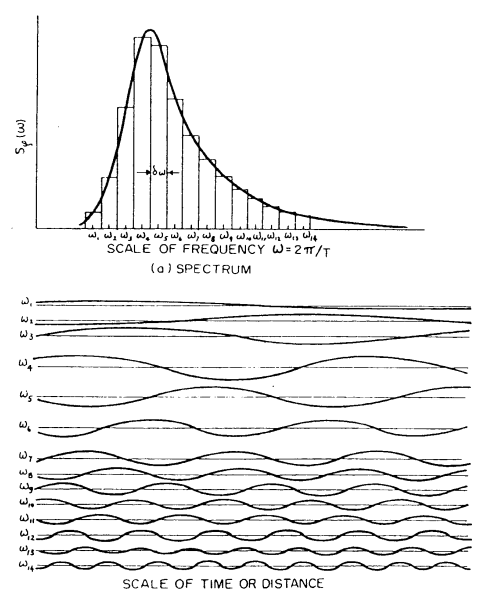
\includegraphics[scale=0.5]{variance_spectrum.png}
  \caption{Variance spectrum}
  \label{fig: variance spectrum}
\end{figure}

It is convenient to define wave components in terms of a function called 
\textit{variance spectrum, $S(\omega)$}. A typical example of a plot of variance
spectrum is shown in figure \ref{fig: variance spectrum}. For any particular 
wave frequency, $\omega_i$, the variance of the wave components for a narrow 
band of frequency, $\delta \omega$, centred on $\omega_i$ is given by:
\begin{equation}
  \langle \zeta_i (t)^2 \rangle = S(\omega_i) \delta \omega
  \label{eq: variance of a narrow band}
\end{equation}
The total variance of the system is given by:
\begin{equation}
  \langle \zeta (t)^2 \rangle = \sum _{i} \langle \zeta_i (t)^2 \rangle = 
  \int _{0}^{\infty} S(\omega) d\omega
\end{equation}
That is, the total variance of the system is obtained by finding the area under
the variance spectrum. Also, as $\delta \omega \to 0$, it means the wave system
is composed of only one frequency which means it becomes a simple harmonic wave. 
The mean value for a wave elevations for a simple harmonic wave is $0$ (wave 
does not increase the mean water level) and the variance is given by:
\begin{equation}
  \langle \zeta_i (t)^2 \rangle = \frac{1}{2} {(\zeta_a)_i }^2
\end{equation}
Applying this is equation \ref{eq: variance of a narrow band}, we get:
\begin{equation}
  \frac{1}{2} {(\zeta_a)_i}^2 = S(\omega_i) \delta \omega
\end{equation}
\begin{equation}
  (\zeta_a)_i = \sqrt{2 S(\omega_i) \delta \omega}
\end{equation}
The above equation is useful to get the amplitude of a component wave within a
frequency band. 

A fair finite-sum model of a unidirectional sea can be obtained by taking about
20 different frequency bands for a single direction. This is because any
particular rectangle in figure \ref{fig: variance spectrum} represents the
variance in that band of frequencies. A regular wave of the indicated finite
amplitude would have the same variance as the infinite number of component
within that band. Hence, the addition of these components (shown at the bottom
of the figure \ref{fig: variance spectrum}) will give a pattern that has the
same total variance and closely resemble the record from which the spectrum was
obtained.

\begin{figure}
  \centering
  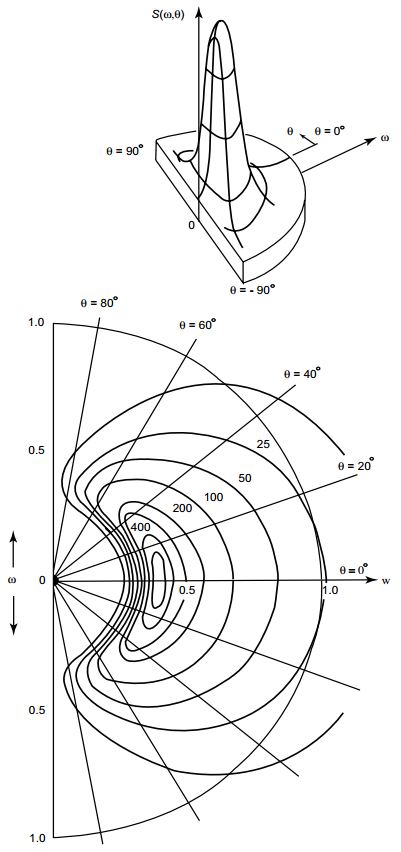
\includegraphics[scale=0.35]{directional_spectrum.png}
  \caption{Directional spectrum}
  \label{fig: directional spectrum}
\end{figure}

A point spectrum does not take into account the direction of propagation of
component waves. A \textit{directional spectrum} gives a more complete
representation of the sea. Figure \ref{fig: directional spectrum} show a typical
example of a directional spectrum. The general equation for the total wave
system of components moving in different direction, $\mu$ is:
\begin{equation}
  \zeta(x,y,t) = \sum _i \sum _j (\zeta_a)_{ij} \cos[k_i (x \cos \mu_j + 
  y \sin \mu_j) - \omega_i t + \epsilon_{ij}]
  \label{eq: equation of ocean wave system}
\end{equation}
And the total variance of the system is:
\begin{equation}
  S = \int_{0}^{\infty} \int_{0}^{2\pi} S(\omega, \mu) d\mu d\omega
  \label{eq: total variance for ocean wave system}
\end{equation}
where $S(\omega, \mu)$ is the function defining the directional spectrum such as
the one shown in figure \ref{fig: directional spectrum}. The following section
looks into various spectral families.

\subsection{Idealized spectral families} \label{Idealized spectral families}

This section describes three idealised point spectrum followed by a section
which describes how to convert point spectrum into a directional spectrum.

\subsubsection{Pierson-Moskowitz spectrum} \label{Pierson-Moskowitz spectrum}
This spectral form requires only one parameter, wind speed, as input and was
developed primarily for oceanographic use. It is intended to represent point
spectrum of a fully developed sea, that is fetch and duration are great, and
there is no contaminating swell from other areas. 
\begin{equation}
  S(\omega) = \frac{\alpha g^2}{\omega^5} 
    e^{ -\beta \big(\frac{g}{V_{\omega}} \big)^4 }
  \label {eq: pierson moskowitz spectrum}
\end{equation}
where:\\
$\omega$ is the frequency in radians/sec\\
$\alpha = 8.10 \cdot 10^{-3}$\\
$\beta = 0.74$ \\
$g =$ acceleration due to gravity in $cm/sec^2$\\
$V_{\omega} =$ wind speed in cm/sec measured 19.5m above the surface.\\

While its oceanographic importance is great, this spectral model is good only
for extreme storm condition and is inappropriate for general use because it is
based on the assumption of full developed sea state reached after an extended
time period of steady wind with no contaminating swell. 

\subsubsection{Bretschneider spectrum} \label{Bretschneider spectrum}
This spectrum takes two input parameters - wave period and wave height. It has
the form:
\begin{equation}
  S(\omega) = \frac{A}{\omega^5} e^{\frac{-B}{\omega^4}}
  \label {eq: bretschneider spectrum}
\end{equation}
where the two parameters $A$ and $B$ depend on the modal frequency, $\omega_m$,
and variance, $S$. The modal frequency is
\begin{equation}
  \omega_m = \bigg[\frac{4}{5}B \bigg]^{\sfrac{1}{4}}
\end{equation}
and total variance is 
\begin{equation}
  S = A/4B
\end{equation}
The International Towing Tank Conference (ITTC, 1978) recommends the use of a
form of Bretschneider spectrum when more specifically appropriate spectral forms
are not known. 
\begin{equation}
  A = 173 \frac{{H_{\sfrac{1}{3}}}^2 }{{T_1}^4}
\end{equation}
\begin{equation}
  B = \frac{691}{{T_1}^4} 
\end{equation}

$H_{\sfrac{1}{3}}$ is the significant wave height and $T_1$ is the time period;
both are inputs.

\subsubsection{JONSWAP spectrum} \label{JONSWAP spectrum}
This spectral function takes two parameters as input - fetch and wind speed. The 
preceding two spectrum models represent open-ocean wave conditions. However, 
this might not always be the case where geographic boundaries limit the fetch in
generating areas. North Sea is such an area and extensive oceanographic
measurements were taken under the Joint North Sea Wave Project (JONSWAP). The
spectral function derived from the recorded data is of the form: 
\begin{equation}
  S(\omega) = \frac{\alpha g}{\omega^{5}} 
  e^{
    {
    \big[ 
      -\frac{5}{4} \frac{\omega}{\omega_m} 
    \big]
    }^{-4}
  }
  \gamma^{
    e^{
        -\frac{(\omega -\omega_m)^2}{2 \sigma^2 {\omega_m}^2}
      }
    }
  \label {eq: JONSWAP spectrum}
\end{equation}
where:\\
$\gamma$ is 3.3\\
$\sigma$ is 0.07 for $\omega < \omega_m$ and is 0.09 for $\omega > \omega_m$\\
$\alpha$ is $0.076 {\tilde{x}}^{-0.22}$\\
$\omega_m $ is $ \sfrac{2 \pi \tilde{f_m} g}{V_{W10}}$ (modal frequency)\\
$\tilde{x}$ is $g \sfrac{x}{{V_{W10}}^2}$\\
$\tilde{f_m}$ is $3.5 {\tilde{x}}^{-0.33}$ \\
$x$ is fetch \\
$V_{W10}$ is wind speed at 10m (32ft) above sea level\\

Note: JONSWAP is simply a form of Bretschneider spectrum, multiplied by a
frequency dependent factor (the $\gamma$ term).

\cite{stansberg2002specialist} provides a more through listing of different wave
spectrum.

\subsubsection{Converting point spectrum to directional spectrum}
\label{Converting point spectrum to directional spectrum}
According to \cite{stansberg2002specialist} even though there are several
unidirectional spectral models, there are only a few multidirectional spectral
models. But, for the multidirectional wave models that are available, the 
data documentation has been lacking or is uncertain. In addition
\cite{stansberg2002specialist} also mentions that for modelling purpose, the
directional characteristics of waves are assumed to be uncoupled from their
spectral properties, and the spectrum of waves travelling within a given range
of headings is taken to be some proportion of that measured at a point. On this
basis, the directional spectrum is of the form:
\begin{equation}
  S(\omega, \mu) = S(\omega) G(\mu)
\end{equation}
$G(\mu)$ is called the \textit{spreading function} and is of the form:
\begin{equation}
  G(\mu) = F(s) \cos^{2s} \frac{1}{2} (\mu - \mu_1)
\end{equation}
where:\\ 
$\mu_1$ is the predominant wave direction  \\
$s$ is an index that determines the width of the directional spread.
\begin{equation}
  F(s) = \frac{2^{2s - 1}}{\pi} \frac{\Gamma^2 (s+1)}{\Gamma (2s + 1)}
\end{equation}
$\Gamma$ is the Gamma function. The function $F(s)$ ensures that the total
variance of the directional spectrum $S(\omega, \mu)$ is same as that of the
point spectrum $S(\omega)$ from which it is derived.\\
\textbf{Note:} Could not find appropriate value for the index $s$ in ITTC 
recommendations.


DNV-GL-H103 \cite{dnv2014recommended} (section 2.2.7) also suggests a similar
approach for converting a point spectrum to a directional spectrum. 
\begin{equation}
  S(\omega, \mu) = S(\omega) G(\mu)
\end{equation}
\begin{equation}
  G(\mu) = \frac{\Gamma(1 + \sfrac{n}{2})}
                {\sqrt{\pi} \Gamma(\sfrac{1}{2} + \sfrac{n}{2})}
           \cos^n (\mu - \mu_p)
\end{equation}
where $\mu_p$ is the prevailing wind direction.

An alternative to the above two formulation is the $15^{th}$ ITTC (1978) 
recommendation mentioned in \cite{lewis1988principles}.
\begin{equation}
  G(\mu) = k \cos^n \mu
\end{equation}
where: \\ 
$\sfrac{-\pi}{2} < \mu < \sfrac{\pi}{2}$\\ 
$n = 2$ \\
$k = \sfrac{2}{\pi}$




\section{Simulation of ocean waves} \label{Simulation of ocean waves}

This section presents a rough structure of the classes and how the data are 
grouped under each class. It also captures the main functions that will be
called when simulating the ocean waves. The aim of this documentation is only to
provide a rough overview and does not aim to mirror the actual implementation. 
The source code documentation will contain the most accurate and in-depth 
description of the classes, its variables. 

The ocean is represented by a surface. The contour of the surface is controlled
by an $n \times n$ matrix of points called the \textit{control points}· The sea
surface is represented by the class \textit{SeaSurface} (section 
\ref{Class SeaSurface}) and the control points are represented by the class
\textit{SeaSurfaceControlPoint} (section \ref{Class SeaSurfaceControlPoint}). 
Random waves are generated on the surface by the interaction of several regular 
waves which are represented by the class \textit{RegularWave} (section 
\ref{Class RegularWave}). The statistically property of the random sea generated 
through the regular waves is controlled by a directional spectrum, which is 
represented by the class \textit{DirectionalSpectrum} (section 
\ref{Class DirectionalSpectrum}). The directional spectrum is a collection of 
point spectrum for each direction ranging from $\sfrac{-\pi}{2}$ to 
$\sfrac{\pi}{2}$.  The directional spectrum contains a table where each row 
represents a point spectrum for a direction and the columns of the table relate 
to each frequency.

\subsection{Class SeaSurface} \label{Class SeaSurface}

The class \textit{SeaSurface} is used to define a square patch of the sea 
surface.

\textbf{Member variables in the class:}
\begin{itemize}
  \item seaPatchSize - size of the square sea patch represented by 
    \textit{SeaSurface}.
  \item seaSurfaceControPoints - an array of points to control the contour of 
    the sea surface.
  \item directionalSpectrum - contains a table of variance values for each
    direction and frequency.
  \item regularWaves - array of all regular waves on the sea surface.
\end{itemize}

\textbf{Methods in the class:}
\begin{itemize}
  \item SetCtrlPointMatSize() - sets the number of control points on the
    surface.
  \item Init()\\
    $>$ Initialise the directional spectrum.\\
    $>$ Create the regular waves in the sea as described below:\\
    $>>$ for each row in directional spectrum (ie: direction):\\
    $>>>$ for each column in directional spectrum (ie: frequency):\\
  	$>>>>$ Get the variance value from the directional spectrum.\\
  	$>>>>$ Calculate the amplitude from variance.\\
    $>>>>$ Generate a random value for wave phase.\\
    $>>>>$ Create a regular wave with the amplitude, phase, frequency and 
          direction.\\
    $>>>>$ Insert the regular wave created into the array regularWaves.
  \item Simulate() \\
    $>$ Initialise time = 0.\\ 
  	$>$ for each point in the array seaSurfaceControlPoints:\\
  	$>>$ for each wave in array regularWaves:\\
  	$>>>$ Calculate displacement due to each wave.\\
    $>>$ Sum the displacements for all waves.\\
    $>>$ Set SeaSurfaceControlPoint.z = sum of displacements.\\
  	$>$ Increment time and continue above loop.
\end{itemize}

\subsection{Class DirectionalSpectrum} \label{Class DirectionalSpectrum}
Class to generate a directional spectrum.

\textbf{Member variable in the class:} 
\begin{itemize} 
  \item countDirections - the number of directions for which point spectrum data 
    will be generated.  
  \item countFrequencies - the number of frequencies bands that will be used for 
    each point spectrum.  
  \item directions - array containing direction angles.
  \item frequencies - array containing the frequency intervals.
  \item spectrum - table containing variance values. Each row corresponds to 
    a direction and each column corresponds to a frequency band.  
\end{itemize}

\textbf{Methods in the class:}
\begin{itemize}
	\item SetCountDirections() - sets value for member variable countDirections.
	\item SetCountFrequencies() - sets value for member variable countFrequencies.
	\item Init()\\
    $>$ Set values for the array directions. \\
		$>$ Set values for the array frequencies. \\
		$>$ For each angle:\\
		$>>$ For each frequency:\\
		$>>>$ Calculate variance $S(\omega)G(\mu)$\\
    $>>>$ Enter the variance into the table spectrum. 
\end{itemize}

\subsection{Class RegularWave} \label{Class RegularWave}
Class to represent a regular wave.

\textbf{Member variables in the class:}
\begin{itemize}
	\item direction - direction of travel of the wave.
	\item phase - the random generated phase value of the wave.
	\item frequency - the circular frequency of the regular wave.
	\item amplitude - the amplitude of the regular wave.
\end{itemize}

\subsection{Class SeaSurfaceControlPoint} \label{Class SeaSurfaceControlPoint}
Class to contain the geographic coordinates of a control point on the sea 
surface. 

\textbf{Member variables in the class:} 
\begin{itemize} 
  \item x - the x coordinate 
  \item y - the y coordinate
  \item z - the z coordinate
\end{itemize}

\subsection{Steps for simulating the random sea} 
\label{Process for simulating the random sea}
\begin{itemize}
	\item Create an object of class SeaSurface.
	\item Set the sea patch dimension.
	\item Call SeaSurface.Init() which in turn calls DirectionalSpectrum.Init().
	\item Call SeaSurface.Simulate().
\end{itemize}

\section{Hydrodynamics} \label{Hydrodynamics}
This section presents a summary of the theory of ASV response motion in waves
and and is mainly based on \cite{lewis1988principles},
\cite{bhattacharyya1978dynamics} and \cite{barltrop2013dynamics}.

ASV in waves experiences oscillatory motions and these motions have six degrees
of freedom that is three transitional components - surge (in longitudinal
direction, x), sway (in transverse direction, y) and heave (in vertical
direction, z), and three angular components - roll (about the longitudinal axis,
x), pitch (about the transverse axis, y) and yaw (about the vertical axis, z).
Of the six motions, only three are purely oscillatory in nature- heave, pitch
and roll. This is because these motions causes a change in the equilibrium
between gravitational force and buoyancy force acting on the vessel resulting in
a restoring force which brings the vessel back to the equilibrium position.
Surge, sway and yaw does not produce a restoring force and hence these motions
are not oscillatory in nature unless the exciting force itself changes direction
and brings it back to the initial state.

At first, this section explores motion in each degrees of freedom independently
of others. That is, for example, it is assumed that the heave motion is not
affect by and does not affect any other motion. In reality this is not true.
Since the ASV is longitudinally asymmetric, the heave motion will also induce
pitching motion. The relationship between each motion in each degrees of freedom
is explored in the section \todo[inline]{To do: Link to section for coupled motion}.

\subsection{Equation of motion}

The equation of motion is based on Newton's second law of motion. For each
transitional motion component, this means that the force acting on the vessel
should be equal the product of mass and acceleration in that direction and for
each angular motion components it means that the moment acting on the vessel
equals the product of mass moment of inertia and angular acceleration. The
general equation of motion for forced oscillation is:
\begin{equation}
  M\ddot{x} + C\dot{x} + Kx = F_0 \cos{\omega t}
  \label{eq: equation of motion}
\end{equation}
where, $x$ is the displacement (Note: $x$ here referrers to displacement in any
particular direction and not just along the $X$-coordinate.). $Kx$ is the
restoring force and $K$ is the hydrostatic stiffness. A body oscillating in a
viscous medium will experience damping force due to dissipation of energy to the
surrounding medium. The term $C\dot{x}$ referrers to the damping force
experienced by the body. $C$ is the damping coefficient and $\dot{x}$ is the
velocity. $M\ddot{x}$ is the inertia force where $M$ is the mass and $\ddot{x}$
is the acceleration. $F_0$ is the magnitude of the periodic force that act on
the body with a frequency $\omege$.

It is more convenient to represent the cyclic force term using complex numbers
as shown below: 
\begin{equation}
  F_0(\omega, t) = F_0 \cos{\omega t} + i F_0 \sin{\omega t} = 
  F_0 e^{i \omega t}
  \label{eq: force for simple harmoic motion}
\end{equation}
The observed value of force at any instant of time is the real part of $F_0$. It
is assumed that the wave excitation forces and the resultant oscillatory motions
are linear and hormonic. Also the frequency of the motion is assumed to be same
as the frequency of wave encounter but with phase lag of $\phi$. Therefore at
any instant of time $t$, the displacement for an encounter wave frequency of
$\omega$ is:
\begin{equation}
  x(\omega, \phi, t) 
  = x_0 \cos(\omega t - \phi) + i x_0 \sin(\omega t - \phi) 
  = x_0 e^{i (\omega t - \phi)}
  \label{eq: displacement for simple harmonic motion}
\end{equation}
\begin{equation}
  \dot{x} = i \omega x_0 e^{i(\omega t - \phi)} = i \omega x
  \label{eq: velocity for simple harmonic motion}
\end{equation}
\begin{equation}
  \ddot{x} = i^2 \omega^2 x_0 e^{i(\omega t - \phi)} = - \omega^2 x 
  \label{eq: acceleration for simple harmonic motion}
\end{equation}
Applying equations \ref{eq: force for simple harmoic motion}, \ref{eq:
displacement for simple harmonic motion}, \ref{eq: velocity for simple harmonic
motion} and \ref{eq: acceleration for simple harmonic motion} in \ref{eq:
equation of motion}, we get:
\begin{equation}
  -M \omega^2 x + i C \omega x + Kx = F_0 e^{i \omega t}
\end{equation}
Therefore:
\begin{equation}
  (-M \omega^2 + i C \omega + K)x = F_0 e^{i \omega t}
\end{equation}
\begin{equation}
  x = \frac{F_0 e^{i \omega t}}{-M \omega^2 + i C \omega + K}
\end{equation}
Or:
\begin{equation}
  x = H F_0 e^(i \omega t)
\end{equation}
where: 
\begin{equation}
  H = \frac{1}{-M \omega^2 + i C \omega + K}
  \label{eq: complex transfer function}
\end{equation}
$H$ is called the \textit{complex transfer function}, because it transfers input
force to output deflection and maintains phase information. The phase lag:
\begin{equation}  
  \phi = \tan^{-1} \bigg( \frac{C \omega}{K - M \omega^2} \bigg)
  \label{eq: phase lag for simple harmonic motion}
\end{equation}  
and amplitude:
\begin{equation}
  x_0 = \frac{F_0}{\sqrt{(K - M \omega^2)^2 + (C \omega)^2}}
\end{equation}

A key point to note is that when the ASV is moving at velocity of $U_0$ at an
angle $\mu$ with respect to wave then the frequency of oscillation will shift
from the wave frequency to the encountered wave frequency. In this case the
$\omega$ term in the above equations should be replaced by encountered wave
frequency,$\omega_e$:
\begin{equation}
  \omega_e = \omega_0 - \frac{\omega_0^2}{g} U_0 \cos \mu 
  \label{eq: encountered wave frequency }  
\end{equation}

\subsection{Exciting force and moment}
\label{Exciting force and moment}

Since the focus of this section is vessel response motion due to waves, the
forces and moments considered are only the fluid forces and moments due to waves
acting on the vessel. Fluid forces and moments can be subdivided into two types
- Froude-Krylov and diffraction excitation. Froude-Krylov excitation force and
moment is obtained by integrating the pressure due to wave on the wetted surface
area of the hull. Froude-Krylov does not consider the effects vessel on the
incident wave. On the other hand, diffraction excitation are forces and moments
due to modification of incident wave due to the presence of the vessel. In cases
where the length of the incident wave is longer than the vessel length, the
diffraction excitation forces and moments will be of small magnitude and hence
is often ignored. 

Froude-Krylov force it obtained by integrating the pressure due to wave along
the wetted surface of the hull. For a regular sea wave, equation \ref{eq:
pressure head variation wrt frequency deep water} in section \ref{Regular sea
waves} provides the formula for pressure head variation due to the wave. The
Froude-Krylov force on the hull can then be obtained as given below:
\begin{equation}
  \int_{\frac{-L}{2}}^{\frac{L}{2}} 
  \int_{\frac{-B}{2}}^{\frac{B}{2}} 
  \rho g \zeta_a e^{k z} \cos (k x - \omega t) 
  \,dx \,dy 
  \label{eq: Froude-Krylov force}
\end{equation}
Since we consider each component motion separately, instead of considering the
total pressure force, we consider the component of the pressure force acting in
component direction. So for hear the above formula will be modified only to take
the vertical component of the pressure force. So, if the surface $\,dx \,dy$ has
an angle $\phi$ with the vertical plane, them the formula for Froude-Krylov
force for heave is: 
\begin{equation}
  \int_{\frac{-L}{2}}^{\frac{L}{2}} 
  \int_{\frac{-B}{2}}^{\frac{B}{2}} 
  \rho g \zeta_a e^{k z} \cos (k x - \omega t) \cos \phi 
  \,dx \,dy 
  \label{eq: Froude-Krylov force for heave}
\end{equation}  
Similarly, for surge and sway motion (which are not harmonic motion) the
Froude-Krylov force can be obtained by taking the component in each direction.

The exciting moments can similarly be calculated by taking the moments of the forces about the axis of rotations. For pitch, the exciting moment about the transverse axis of the ASV is:
\begin{equation}
  \int_{\frac{-L}{2}}^{\frac{L}{2}} 
  \int_{\frac{-B}{2}}^{\frac{B}{2}} 
  \rho g \zeta_a e^{k z} \cos (k x - \omega t) \cos \phi x
  \,dx \,dy 
\end{equation}
The moments for roll and yaw can also be calculated similarly.

\section{Simulation of vessel motion in waves} 
\label{Simulation of vessel motion in waves}

This section describes{ simulation of vessel motion in waves. The first step is
to generate all the waves and this is described in section \ref{Simulation of
ocean waves}. After generating the ocean waves the vessel response motion is
calculated for each wave for each heading angle and speed. The results are then
saved in a series of tables. 

\subsection{Calculating motion response for each wave}
\label{Calculating motion response for each wave}

\begin{algorithmic}
  \FOR {each regular wave in the simulation field} 
    \FOR {each heading angle between 0 and 360 degree}
      \FOR {each vessel speed} 
        \STATE calculate encounter frequency 
        \STATE calculate total pressure by integrating pressure below the wetted
        surface area 
        \STATE calculate total added mass by integrating added mass along the
        length of ASV 
        \STATE calculate total damping coefficient by integrating damming 
        coefficient along the length of ASV 
        \STATE calculate hydrostatic stiffness 
        \STATE calculate response amplitude 
        \STATE calculate response motion phase lag
      \ENDFOR
    \ENDFOR
  \ENDFOR
\end{algorithmic}

\subsection{Calculating total pressure force}
\label{Calculating total pressure force}
The total pressure force is calculated by integrating the pressure along the
wetted surface area. The wetted surface area can be found by finding the
intersection of the hull surface with the wave profile. 

\begin{algorithmic}
  \STATE let $totalPressureForce = 0$ 
  \FOR {each element in the ASV hull mesh}
    \STATE find if the mesh is above, below or intersecting the wave profile.
    \IF{mesh above wave profile}
      \STATE continue
    \ELSIF{mesh below wave profile}
      \STATE get mesh area and centroid 
    \ELSE
      \STATE find intersection of mesh with wave profile
      \STATE find area and centroid for mesh area below the wave profile.
    \ENDIF
    \STATE calculate the pressure force using formula \ref{eq: Froude-Krylov 
    force}. The pressure force should use the centroid of the the patch for 
    coordinate location and area of the patch to get the force.
    \STATE $totalPressureForce += pressureForceOnMesh $ 
  \ENDFOR
\end{algorithmic}

\subsection{Calculating total added mass and total damping coefficient}
\label{Calculating total added mass}
The total added mass and total damping coefficient is calculated using strip
theory. The full length of the ASV will be divided longitudinally into strips
and the added mass and damping coefficients will be calculated for each strip.
Sum of added mass of all strips will give the total added mass of the vessel and
sum of damping coefficients of all strips will give the total damping
coefficient.

\subsection{Calculating response amplitude}
\label{Calculating response amplitude}
Response amplitude is calculated using equation \ref{eq: equation of motion} but
instead of solving the equation of motion for each degree of freedom separately,
we will use matrices to simultaneously solve the equations of motion for all
degrees of freedom. 

$M$ : Mass matrix
\[
\begin{bmatrix}
  $\Delta$ & 0 & 0 & 0 & $+\Delta z_c$ & 0 \\
  0 & $\Delta$ & 0 & $-\Delta z_c$ & 0 & $+\Delta x_c$ \\
  0 & 0 & $\Delta$ & 0 & $-\Delta x_c$ & 0 \\
  0 & $-\Delta z_c$ & 0 & $I_{44}$ & 0 & $-I_{46}$ \\
  $+\Delta z_c$ & 0 & $-\Delta x_c$ & 0 & $I_{55}$ & 0 \\
  0 & $+\Delta x_c$ & 0 & $-I_{46}$ & 0 & $I_{66}$
\end{bmatrix} 
\]
where: \\
$\Delta$ : is total mass of vessel \\
$I_{44}, I_{55}, I_{66}$ : are moments of inertia around the longitudinal,
transverse and vertical axis of the ASV. \\
$I_{46} = I_{64}$ : is roll - yaw product of inertia.\\
$x_c, z_c$ : are the coordinates of centre of gravity of the ASV. The ASV is
assumed to be transversely symmetric and hence $y_c = 0$

$C$ : Damping matrix
\[
\begin{bmatrix}
\end{bmatrix} 
\]

$K$ : Stiffness matrix
\[
\begin{bmatrix}
\end{bmatrix} 
\]

$F$ : Force vector
\[
\begin{bmatrix}
\end{bmatrix} 
\]

$x$ : Displacement vector
\[
\begin{bmatrix}
\end{bmatrix} 
\]


% Breakpage and set bibliography
\clearpage
% Add References to table of contents
\addcontentsline{toc}{section}{References}
% Add the references
\bibliographystyle{ieeetr}
\bibliography{reference}

%\listoftodos
\end{document}
